\documentclass[12pt ,a4paper ]{article}

\usepackage[utf8]{inputenc}
\usepackage[T1]{fontenc}      % caractères français
\usepackage[french]{babel}  %langue
\usepackage[left=2.3cm,right=2.5cm,bottom=2cm,top=2.3cm]{geometry}   % marges
\usepackage{verbatim}
\usepackage{float}
\usepackage{graphicx}         % images
\usepackage{verbatim}
\usepackage{multicol}
\usepackage{titlesec}

\usepackage[hyphens]{url}
\usepackage{hyperref}
\hypersetup{
    colorlinks=true,
    linkcolor=black,
    urlcolor=blue,
}

\urlstyle{same}


                           
\begin{document}
	\begin{titlepage}
		
		\vspace{0.5cm}
		\begin{center}		
			{\Large  Master 1 Informatique}
		\end{center}
		\vspace{1cm}
		
		\rule{1\linewidth}{1.1pt}\newline   %regle
		\begin{center}
			 {\Huge \textbf{Rapport de Projet : Neural Network And Learning}}
		\end{center}
		\rule{1\linewidth}{1.1pt} \\
		
		\begin{center}
		\begin{LARGE}
		\textbf{Sujet :} \\\vspace{0.6cm}  Construction d'un classificateur de photo de scènes naturelles
		\end{LARGE}
		\end{center}
		
		\vspace{0.5cm}
		\begin{center}	
				\begin{Large}
				Yann MARTIN D'ESCRIENNE \\ 
				Yohann TOGNETTI \\ 
				\end{Large}
		\end{center}
		\vspace{6cm}
		
		\begin{center}
			{\large « Année universitaire 2020 - 2021 »}
		\end{center}
		

\end{titlepage}

\newpage
\tableofcontents 
				
\newpage


\begin{multicols}{2} 
\section{Présentation générale du projet}
		Dans le cadre de notre cours de Neural Network and Learning, il nous a été demandé d'effectuer un projet impliquant une intelligence artificielle travaillant sur des images. Celle-ci a pour but de construire un classificateur de photo de scènes naturelles comme ceux qu’on pourrait intégrer dans un appareil photo intelligent qui à chaque prise de photo va taguer l’image avec le nom d’une catégorie qui y correspond. 
	
		
\section{Descriptif du sujet et ses finalités}
\subsection{Descriptif du sujet}
	Ainsi, pour entrer dans les détails le but qui est de "taguer l'image" correspond au fait de la catégoriser grâce à un classificateur entrainé possédant les catégories de scènes naturelles désirées. Pour cela avons dû utiliser un réseau neuronal convolutif étant donné que nous traitons des images. Une fois la réponse du classificateur reçue, elle correspond initialement à un entier, nous avions donc le devoir de le convertir en tag correspondant au nom de la catégorie trouvée. \\
	
	
	L'affichage du résultat doit se faire à l'aide d'une méthode \textit{predict} qui prend en entrée le chemin de fichier d’une image et une chaine de caractères 'mode' qui renvoie le nom de la catégorie correspondant à l'image si \textbf{mode='category'} où un vecteur de probabilités si \textbf{mode='probabilities'} ou chaque éléments du vecteur indique la probabilité que l'image appartienne à la catégorie correspondante.

\subsection{Les catégories}
Celles-ci sont au nombre de 6, chacune correspond à une catégorie de paysage ou de scène naturelle de la liste suivante : 

\bigskip
\begin{itemize}
\item buildings
\item forest
\item glacier
\item mountain
\item sea
\item street
\end{itemize}

\bigskip
\textit{Building} correspond ainsi à des bâtiments comme une maison ou un immeuble qui se trouve généralement dans une ville. \textit{Forest} comme son nom l'indique correspond à un paysage forestier avec la présence ou non d'animaux. 
\textit{Glacier} quant à lui représente une montagne enneigée ou bien un glacier ou morceaux de glace de la banquise, cette catégorie est extrêmement corrélée avec \textit{Moutain} car celle-ci correspond à une montagne pouvant parfois aussi être enneigé. Le découpage n'est pas toujours pertinent et encore plus ici, nous en parleront dans la section \textit{Description des données}. \textit{Sea} représente les décors marins en général, que ce soit une plage, la mer avec ou sans terre ferme, ou bien même un décor sous-marin, tout cela va dans cette catégorie. Enfin la catégorie \textit{Street} met en avant une rue, qui peut donc facilement se rapprocher de \textit{building} étant donnée la présence quasi-permanente de bâtiments dans une rue, on y trouve souvent des passant et des voitures.  

\section{Jeux de données}
Les jeux de données se divisent en deux groupes : le jeu de données d'entrée correspondant à ce que l'IA va utiliser pour s'entrainer et celui de test sur lequel les mesures seront effectuées. Tout deux proviennent du site du SemEval. 

\subsection{Structure des jeux de données}
\noindent Ce sont tout deux des documents XML possédant la structure suivante (simplifiée) :  

\begin{figure}[H]
\begin{center}
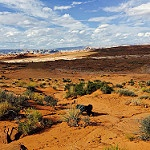
\includegraphics[scale=0.55]{3808.jpg}
\caption{\small{structure du fichier XML}}
\end{center}
\end{figure}

\subsection{Modification des jeux de données}
Suite à notre implémentation de notre IA qui sera décrite dans le chapitre suivant, de nombreux problèmes nous ont forcés à ajouter nous même des phrases dans le jeu de données d'entrainement.\\

En effet notre IA répond de la présence ou non de chaque couple E\#C pour chaque combinaison d'entité E et catégorie C. Cela se traduit par une nécessité de nombreuses données appartenant à chacun des couples pouvant apparaitre afin d'obtenir une fonction d'évaluation optimale. Dans le cas contraire le résultat est rarement celui attendu, il nous a donc fallu compléter le jeu de données.

\paragraph{}
Environ 350 phrases ont été ajoutées, toutes sont la section 'sentences' d'\textbf{ID 198}. Certaines proviennent d'avis de consommateur sur les ordinateur portables les plus commentés sur Amazon (en anglais), notamment pour les phrases portant sur les clavier, écran, pavé tactile et batterie, qui sont de manière générale beaucoup cité dans une revue de produit. Nous avons rédigés le reste pour les catégories plus complexe et moins abordées. Par exemple la qualité des lecteurs DVD ou bien l'ergonomie des OS. Cela s'éloigne d'un cas réel mais reste tout de même nécessaire au bon apprentissage de l'IA. \\ 

\noindent \textit{Remarque : } Il est à noté que certain couple n'apparaissent ni dans les données d'entrainement, ni dans les données de test. Par simplification, ces couples ont été ignorés et aucunes phrases n'est étiquetées avec.

\begin{figure*}[th]
    \begin{center}
        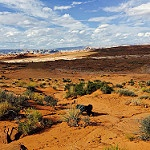
\includegraphics[width=1\textwidth]{3808.jpg}
    \end{center}
\caption{\small{dataframe du fichier XML}}
\end{figure*}
\newpage
\section{Implémentation de l'algorithme}
Notre algorithme est développé en python. Il se divise en 4 fichiers de code ayant chacun un rôle précis dans l'implémentation de l'algorithme d'apprentissage. 

\subsection{DataInitializer.py}
Ce fichier permet de lire un documents XML du jeu de données et regroupe les informations essentielles dans un dataframe de la librairie \textit{panda}. Chacune des phrases correspondent à une ligne dans le dataframe. \\

\noindent Il vient tout d'abord récupérer l'ID et le texte de chaque phrase. \\

\noindent Ensuite il récupère chaque couple E\#C et transforme le tout en un vecteur binaire ayant des 1 uniquement aux colonnes correspondant au couple comme sur l'image ci-dessus encadré en rouge. Étant donné le nombre de couples possible, il s'agit d'une vecteur à 197 dimensions comportant majoritairement des 0.\\

\noindent Finalement, le programme récupérera la polarité de chaque couple E\#C et conclue une polarité générale de la phrase selon les règles suivantes :
\begin{enumerate}
\item \textbf{\small{neutral + X = X, X une polarité. }}
\item \textbf{\small{positive + negative = mixed.}}
\item \textbf{\small{mixed + X = mixed, X une polarité.}}
\end{enumerate}

\noindent Cette polarité général est ensuite convertie en entier:

\noindent \textbf{0=negative, 1=positive, 2=neutral, 3=mixed.}

\subsection{PreProcessing.py}
Ce fichier permet d'effectuer un pré traitement sur les textes du premier data frame afin de facilité le travail d'apprentissage de l'IA. Il s'appuie notamment sur la librairie \textit{nltk}.\\

\noindent Tout d'abord le texte va être mit en minuscule afin de ne pas différencier des mots n'ayant pas la même casse. Ensuite chacun de ses mots (y compris la ponctuation) va être transformé en \textbf{« token »}. De ces tokens sera retiré la ponctuation ainsi que ce que l'on appelle les \textbf{STOPWORDS}. Ce sont les mots n'ayant pas de grande valeurs syntaxique comme les déterminants, adjectifs possessifs, conjonctions de coordination, verbes communs (être, avoir)...\\

\noindent L'étape suivante consiste à effectuer une \textbf{lemmatisation} sur chacun des tokens. La lemmatisation est un traitement lexical qui consiste à appliquer aux verbes, substantifs, adjectifs... un codage renvoyant à leur entrée lexicale commune, leur « forme canonique ».\\\\

\noindent \textit{Exemple :}\\
Les / la\\
étoiles /étoile\\
claires / clair\\
luisent / luire\\
noire / noir\\

\noindent Voici une image des phrases du dataframe précédent où celles-ci ont été pré-traitées : 
\begin{figure}[H]
    \begin{center}
        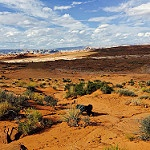
\includegraphics[scale=0.62]{3808.jpg}
    \end{center}
\caption{\small{Phrases pré-traitées}}
\end{figure}

\subsection{Classify.py}
Ce fichier a pour fonction de créer un classificateur pour chaque classes qui possèdent des données pour s'entrainer. L'intégralité de ce fichier utilise principalement la librairie \textit{sklearn} qui est une librairie complète pour l'apprentissage d'une IA.\\

\noindent \textit{Remarque : } 
Comme dit précédemment , certaines classes n'étant pas existante dans les données d'entrainement (ET dans les données de test), elles n'ont donc pas de classificateur attitré.\\

La première opération à faire pour pouvoir créer un classificateur, est de transformer les phrases en vecteurs. Pour cela, nous avons utilisé \textbf{TfidfVectorizer} de la librairie sklearn. Au niveau des paramètres, nous avons décidé d'utiliser\textbf{ la norme "l2"} et d'utiliser des \textbf{ngram entre 1 et 8}. Une fois créé nous avons entrainé ce vectoriseur avec les commentaires de notre jeu de d'entrainement.\\

Ensuite, nous pouvons commencer la classification. Pour celle-ci nous avons décidé d'utiliser la méthode \textbf{one-versus-rest} (« une contre le reste »). Cette méthode consiste à traiter chaque classe indépendamment des autre. Chaque classe représente ici un de nos couple E\#C.\\

Dû au peu de données présente pour certaine classe, et l'effort pour en ajouter d'autre étant trop élevé, nous avons eu recourt à un algorithme d'échantillonnage pour augmenter les classes minoritaires. Cet algorithme n'est autre que \textbf{ADASYN} (Adaptive Synthetic). A partir des données existantes (au moins 5 ici), l'algorithme va en créer d'autre en utilisant le principe des \textit{« K plus proche voisins »}. L'image ci-dessous montre l'efficacité d'ADASYN.\\

\begin{figure}[H]
    \begin{center}
        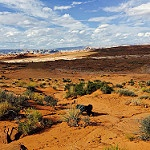
\includegraphics[scale=0.62]{3808.jpg}
    \end{center}
\caption{\small{L'algorithme ADASYN}}
\end{figure}

Après avoir fait cela, il nous reste plus qu'à entrainer chacun des classificateurs. Nous avons utiliser donc utilisé \textbf{OneVsRestClassifier} avec comme\textbf{ solver "sag"}, un \textbf{poids équilibré entre chaque classe} et un nombre d'\textbf{itération maximum de 1000}. Afin de pouvoir réutiliser ces classificateurs pour notamment évaluer une phrase à la volée, nous les stockons dans un dictionnaire ayant pour clé la catégorie et pour valeur le classificateur de cette catégorie.\\

La dernière fonction de cette classe est la prédiction un dataframe test. Pour ce faire, à l'aide du vectoriseur et des classificateurs, il nous suffit de pré-traiter et vectoriser chaque phrases et d'appeler pour chacune l'intégralité des classificateurs stockés dans le dictionnaire pour prédire à quelles classes (ou couple E\#C) appartient chaque commentaire.

\subsection{PlotResult.py}
Ce fichier utilise la libraire \textit{matplotlib} de python. Il permet de mettre en place la représentation graphiques des résultats obtenus. Les données sont récupérées lors de la classification du fichier précédent, puis sont misent dans des diagrammes en barre. Cela permet d'avoir une vision générale mais rapide des différents score évalués. En effet il y a beaucoup de classes différentes et un rapport de classification détaillés pour chacune d'elle ne serais pas pertinent.

\begin{figure*}[t]
    \begin{center}
        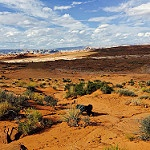
\includegraphics[width=1.15\textwidth]{3808.jpg}
    \end{center}
    \caption{F1-score de chaque classe pour 0 et 1}
\end{figure*}
\newpage
\section{Résultat obtenus}
Il est à noter que les résultats peuvent être légèrement différent à chaque appel du programme ainsi les graphiques qui vont suivre ne sont pas forcément absolus. 

\subsection{Résultat général}
Il est facilement remarquable sur la \textit{figure 5} que la valeur 0 (donc l'absence du couple E\#C) possèdent un bien meilleur score que la valeur 1. En effet un commentaire parlant d'un clavier uniquement ne va pas parler d'un écran ou d'une souris, ce qui créer un nombre conséquent de données négative (c-à-d 0) pour chaque classes. Il est alors plus facile pour l'IA de déterminé si la phrase n'appartient pas à un couple que l'inverse.\\

On constate effectivement que le f1-score des valeurs 1 de chaque classe est assez variable et atteins parfois même 0\%. Cela s'explique avec deux raisons: 
 
\noindent Soit par une \textit{précision} de 0\%, car certain couple dans les données de test n'ont qu'une apparition ce qui rend le résultat binaire ou bien simplement par l'échec de l'IA à classer correctement les phrases (les justifications de cette lacune sera expliquée dans l'analyse du résultat suivant). 

\noindent Soit par un \textit{recall} faible, car l'IA peut facilement trouvé la bonne entité mais pas la bonne catégorie et vis-versa, et cela se traduit par une réduction du recall et donc du f1-score.\\

Comme dit précédemment, la valeur du f1-score des valeurs 0 est très élévé, environ 95\%, ainsi ne nous y attarderont pas plus que ça dans les analyses suivantes et nous concentrerons plus sur les résultats et scores obtenus pour les valeurs 1.

\begin{figure*}[t]
    \begin{center}
        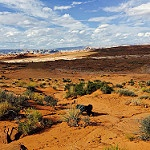
\includegraphics[width=1.15\textwidth]{3808.jpg}
    \end{center}
    \caption{précision et support de la valeur 1}
\end{figure*}
\newpage
\subsection{Résultat pour la valeur "1"}
On remarque premièrement que les précisions de chaque couple E\#C ne sont pas homogène. Cela s'explique par la différence majeure entre chaque entités et les catégories qui s'y rapportent. En effet il est beaucoup plus simple et parler de l'ergonomie d'une souris (ou d'un pavé tactile) que de l'ergonomie d'un OS, ce qui explique par exemple l'écart de précision entre ces deux couples. \\

De plus, certain couples possèdent un jeu de données qui se veut parfois peu ressemblant entre chaque élément y appartenant. Par exemple, dans le commentaire d'un clavier, il y aura beaucoup de chance de trouver les mots "touche","clavier" ou bien "pavé numérique", ce qui focalise l'IA sur certain éléments clés et ressort de tout cela une bonne précision. Mais par exemple, le couple \textit{COMPANY\#GENERAL} peut très bien parler de \textit{Windows} comme d'\textit{Apple}, \textit{Dell} , \textit{toshiba} ... de mille et une façon, ce que l'IA a du mal à assimiler. \\

Enfin, une relation logique apparait entre le support (nombre d'éléments) et la précision. Moins on a de données plus la précision est extrême (0\% ou bien 100\%) car soit l'IA a tout juste, soit tout faux. Au contraire, lors d'une présence d'un nombre de données assez conséquent (environ 10), la précision tend à dépasser les 50\% ce qui pourrait être plus représentatif du niveau de classification. Typiquement, le nombre de données le plus élevé (214) est celui du couple \textit{LAPTOP\#GENERAL} (ce qui est assez logique en soit) et il possède une précision de 71\%.

\begin{figure*}[t]
    \begin{center}
        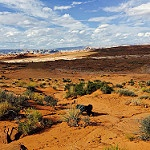
\includegraphics[width=1.15\textwidth]{3808.jpg}
    \end{center}
    \caption{score par entités}
\end{figure*}
\newpage
\subsection{Résultat par entités}
Suite à de nombreux tests sur des classifications de phrases, nous avons remarqué que l'IA se trompe parfois dans le ou les couple E\#C mais arrive tout de même à reconnaitre la ou les entités E qui sont ciblés dans la phrase. Nous avons donc regroupé par entité pour plus de pertinence et avons calculé la \textit{precision}, le \textit{recall} et le \textit{f1-score} de chacune.\\

Là encore attention, malgré le regroupement par entité, certaines n'ont qu'un seule données, ce qui explique les scores à 50\%. De plus, nous avons récupéré la macro-moyenne (moyenne brute) et non la moyenne pondérée car celle-ci est figé à 99\% pour toutes les entités (dû à grand nombre de cas à 0 et très peu d'erreur de l'IA dessus comme expliqué précédemment), il n'est donc pas intéressant de faire une étude dessus. Cette macro-moyenne se retrouve donc à cette valeur lorsqu'il n'y a qu'une donnée pour la valeur 1 et que l'IA ne retrouve pas la bonne entité E suivant le simple calcule suivant : 

\begin{equation}
(99 + 0) / 2 \simeq 50 \%.
\end{equation}

Mis à part ces cas précis, les scores obtenus sont relativement corrects et on peut facilement affirmer que l'IA arrive à reconnaitre les entités cible d'un commentaires. Toutefois, nous avons remarqué que lorsque la phrase aborde différentes entités de manière brève, par exemple \textit{"L'ordinateur est cool, le clavier et le son sont correct mais l'affichage est magnifique"}, la classification de toutes ces entités semble très difficile pour l'IA. \\

\begin{figure*}[t]
    \begin{center}
        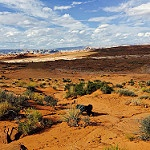
\includegraphics[width=1.15\textwidth]{3808.jpg}
    \end{center}
    \caption{score de la polarité}
\end{figure*}
\newpage
\subsection{Résultat de la polarité}
Tout d'abord voici le nombre de données de base par polarité :
\begin{itemize}
\item negative : 768
\item positive : 917
\item neutral : 430
\item mixed : 46
\end{itemize}
\medskip
On constate que la \textit{précision}, le \textit{recall} et le \textit{f1-score} sont relativement proche pour chaque polarité ce qui ne souligne pas de problème particulier dans une classe. 
Il est notable que \textit{positive} et \textit{negative} sont les deux  classes qui comportent le plus de données, il est donc normal que leur score soit les plus élevés. \\

Le fait d'avoir un commentaire positif semble d'ailleurs plus facile à détecter qu'un commentaire négatif. Cela s'explique par le fait que souvent, un commentaire négatif consiste en l'énumération des défauts de l'ordinateur sans forcément de mot clé signifiant une insatisfaction ou un mécontentement, l'IA à donc plus de mal à déterminé si cela est négatif (une énumération de fait pouvant être neutre). \\

Ainsi, la polarité \textit{neutral} peut ressortir également de plusieurs tournure de phrase. Aucun mot clé n'est propre à un avis neutre, ce qui rend plus difficile sa classification et lui donne des score relativement médians. \\

Finalement, la polarité \textit{mixed} possède le score le plus bas car d'une part, le jeu de données est très faible relativement aux autres, mais également, c'est la polarité la plus dure à classifiée et n'existe pas réellement. Nous l'avons créer dû à la simplification que nous avons faite d'avoir une polarité générale et non propre à chaque couples E\#C. Il est donc évident qu'elle n'est pas absolue et consiste à la fusion d'un avis positif et négatif. 

\newpage
\section{Les améliorations possibles}
Dans cette nous allons voir ce que nous aurions pu améliorer dans notre projet.

\subsection{Les classe}
Le plus gros problème de notre sujet sont les classes qui ont été choisies pour le jeu de données, il y en a beaucoup trop (126) dont la plupart qui sont similaire. Avec plus de temps, il aurais été préférable de refaire la plupart des classes sans garder la forme \textit{entité\#categorie}. Car pour des phrase comme \textit{"L'ordinateur est rapide"}, cela veux dire que l'on parle de plusieurs entités comme DISPLAY, CPU, LAPTOP, GRAPHICS, SOFTWARE, ... et pour chacune, des catégories GENERAL et OPÉRATION PERFORMANCE.\\
Pour corriger cela, le mieux aurait été de faire moins de classe mais avec des spécificité plus générale (comme \textit{"composant", "service"..}) ce qui aurais permit de mieux classifier et d'être plus précis.

\subsection{Le jeu de données}
La deuxième amélioration majeure que l'on aurais pu faire aurait été d'ajouter plus de données à notre jeu d'entrainement ou bien même avoir un jeu de données plus conséquent et plus orienté dans la conception choisie avec les différents couples. Cet élément est ce qui nous à poser le plus de problème dans le projet.

\subsection{Les marques et modèles}
Quand on parle de matériels informatique, il arrive souvent de parler d'un modèle spécifique. Pour les processeur le vocabulaire CPU ou processeur ne vas pas toujours être employé, l'utilisateur utilisera plutôt les mots \textit{"i7"} ou \textit{"intel"} ou encore\textit{"ryzen"} qui sont des modèle des processeurs. Cela se retrouve sur plusieurs entités différentes. Il aurait été possible de changer les Tokens des modèles spécifiques lors de leur récupération par un mot plus général, si nous reprenons l'exemple il serait possible de tout remplacer par le mot \textit{"processeur"}. Cela aurait surement amélioré l'efficacité de l'IA dans sa classification.

\subsection{La polarité}
Avec le choix de faire une polarité générale par phrase, il y a un travail assez intéressant qui s'est retrouvé écarté. En effet, il aurait été intéressant d'essayer de faire une polarité pour chaque couple trouvées comme demandé dans le SemEval. Pour cela, il aurais fallu réussir à isoler le morceau de phrase qui a permit de détecter la classe. Puis à partir de ce sous-ensemble, faire de nouveau une classification sur la polarité. Par manque de temps et d'expérience, cette isolation de sous-ensemble par couple fut trop complexe, il aurai fallu partir d'une IA avec une classification déjà presque parfaite afin de ne pas sélectionner une sous-ensemble incohérent. Ce qui n'était pas notre cas. 

\end{multicols}
\newpage
\section{Conclusion}
La mise en place de ce projet fut un challenge. En effet, il nous a fallu construire nous même chaque couple entité-catégorie et utiliser la classification \textit{one-vs-rest} que nous ne maitrisions pas du tout.\\
La partie la plus simple fut de pré-traiter le texte et de récupérer les données depuis le document XML et d'en faire des diagrammes. Sûrement dû à nos connaissances acquises au court de notre cursus et de cette matière. \\
Une fois la classification mise en place, nous avons heurter le problème du manque de données qui dans un premier temps ne fût pas corriger par l'algorithme \textit{ADASYN,} car le jeu données étant vraiment trop pauvre pour certaine classes celui-ci en créait de nouvelles un peu diverse (l'IA répondait toujours non aux tests pour les classes concernées). Il nous a donc fallu ajouter énormément de données ce qui est dommage car nous n'en avons tiré aucun apprentissage.\\
Plus généralement, ce projet nous aura permit de nous familiariser avec les librairies \textit{sklearn} et \textit{nltk}, d'apprendre de nouvelles façon de classifier lorsque plusieurs classes peuvent apparaitre pour un même cas, mais également de solutionner le problème du dés-équilibrage des classes et des valeurs et finalement de manipuler l'apprentissage d'une IA avec des données textuelles et leur pré-traitement.

\section{Références}
\begin{itemize}
\item Top Rated in Laptop Computers  :\\ \url{https://www.amazon.com/pcr/Top-Rated-Laptop-Computers-Reviews/565108}%
\item The “Imbalanced classification problem” :\\ \url{https://medium.com/@bluedme_tech/comment-traiter-les-probl%C3%A8mes-de-classification-d%C3%A9s%C3%A9quilibr%C3%A9e-en-machine-learning-8c3bc95ca25b}%
\item Deep dive into multi-label classification :\\ \url{https://towardsdatascience.com/journey-to-the-center-of-multi-label-classification-384c40229bff}%
\item Tutoriel TAL pour les débutants :\\ \url{https://www.actuia.com/contribution/victorbigand/tutoriel-tal-pour-les-debutants-classification-de-texte/}%
\item SemEval-2015 Task 12 :\\ \url{https://alt.qcri.org/semeval2015/task12/index.php?id=data-and-tools}%
\item WIKIPEDIA FR :\\ \url{https://fr.wikipedia.org/wiki/Wikip%C3%A9dia:Accueil_principal}%
\end{itemize}




\end{document}